\documentclass{article}
\usepackage[ngerman]{babel}
\usepackage[margin=2cm]{geometry}
\usepackage{amsmath, amssymb, amsfonts}
\usepackage{tikz}
\usepackage{graphicx}
\usepackage{fancyhdr}

\usepackage{tcolorbox} %Umgebung mit farbigem Hintergrund

\graphicspath{{../../}}
%Seitenstil modifizieren
\pagestyle{fancy}% eigenen Seitestil aktivieren}
\fancyhf{}% Alle Felder loeschen

\fancyhead[L]{
\begin{tabular}[b]{l}
Lernstandsübersicht\\
Mathematik\\
Klasse 9
\end{tabular}}
\fancyhead[R]{
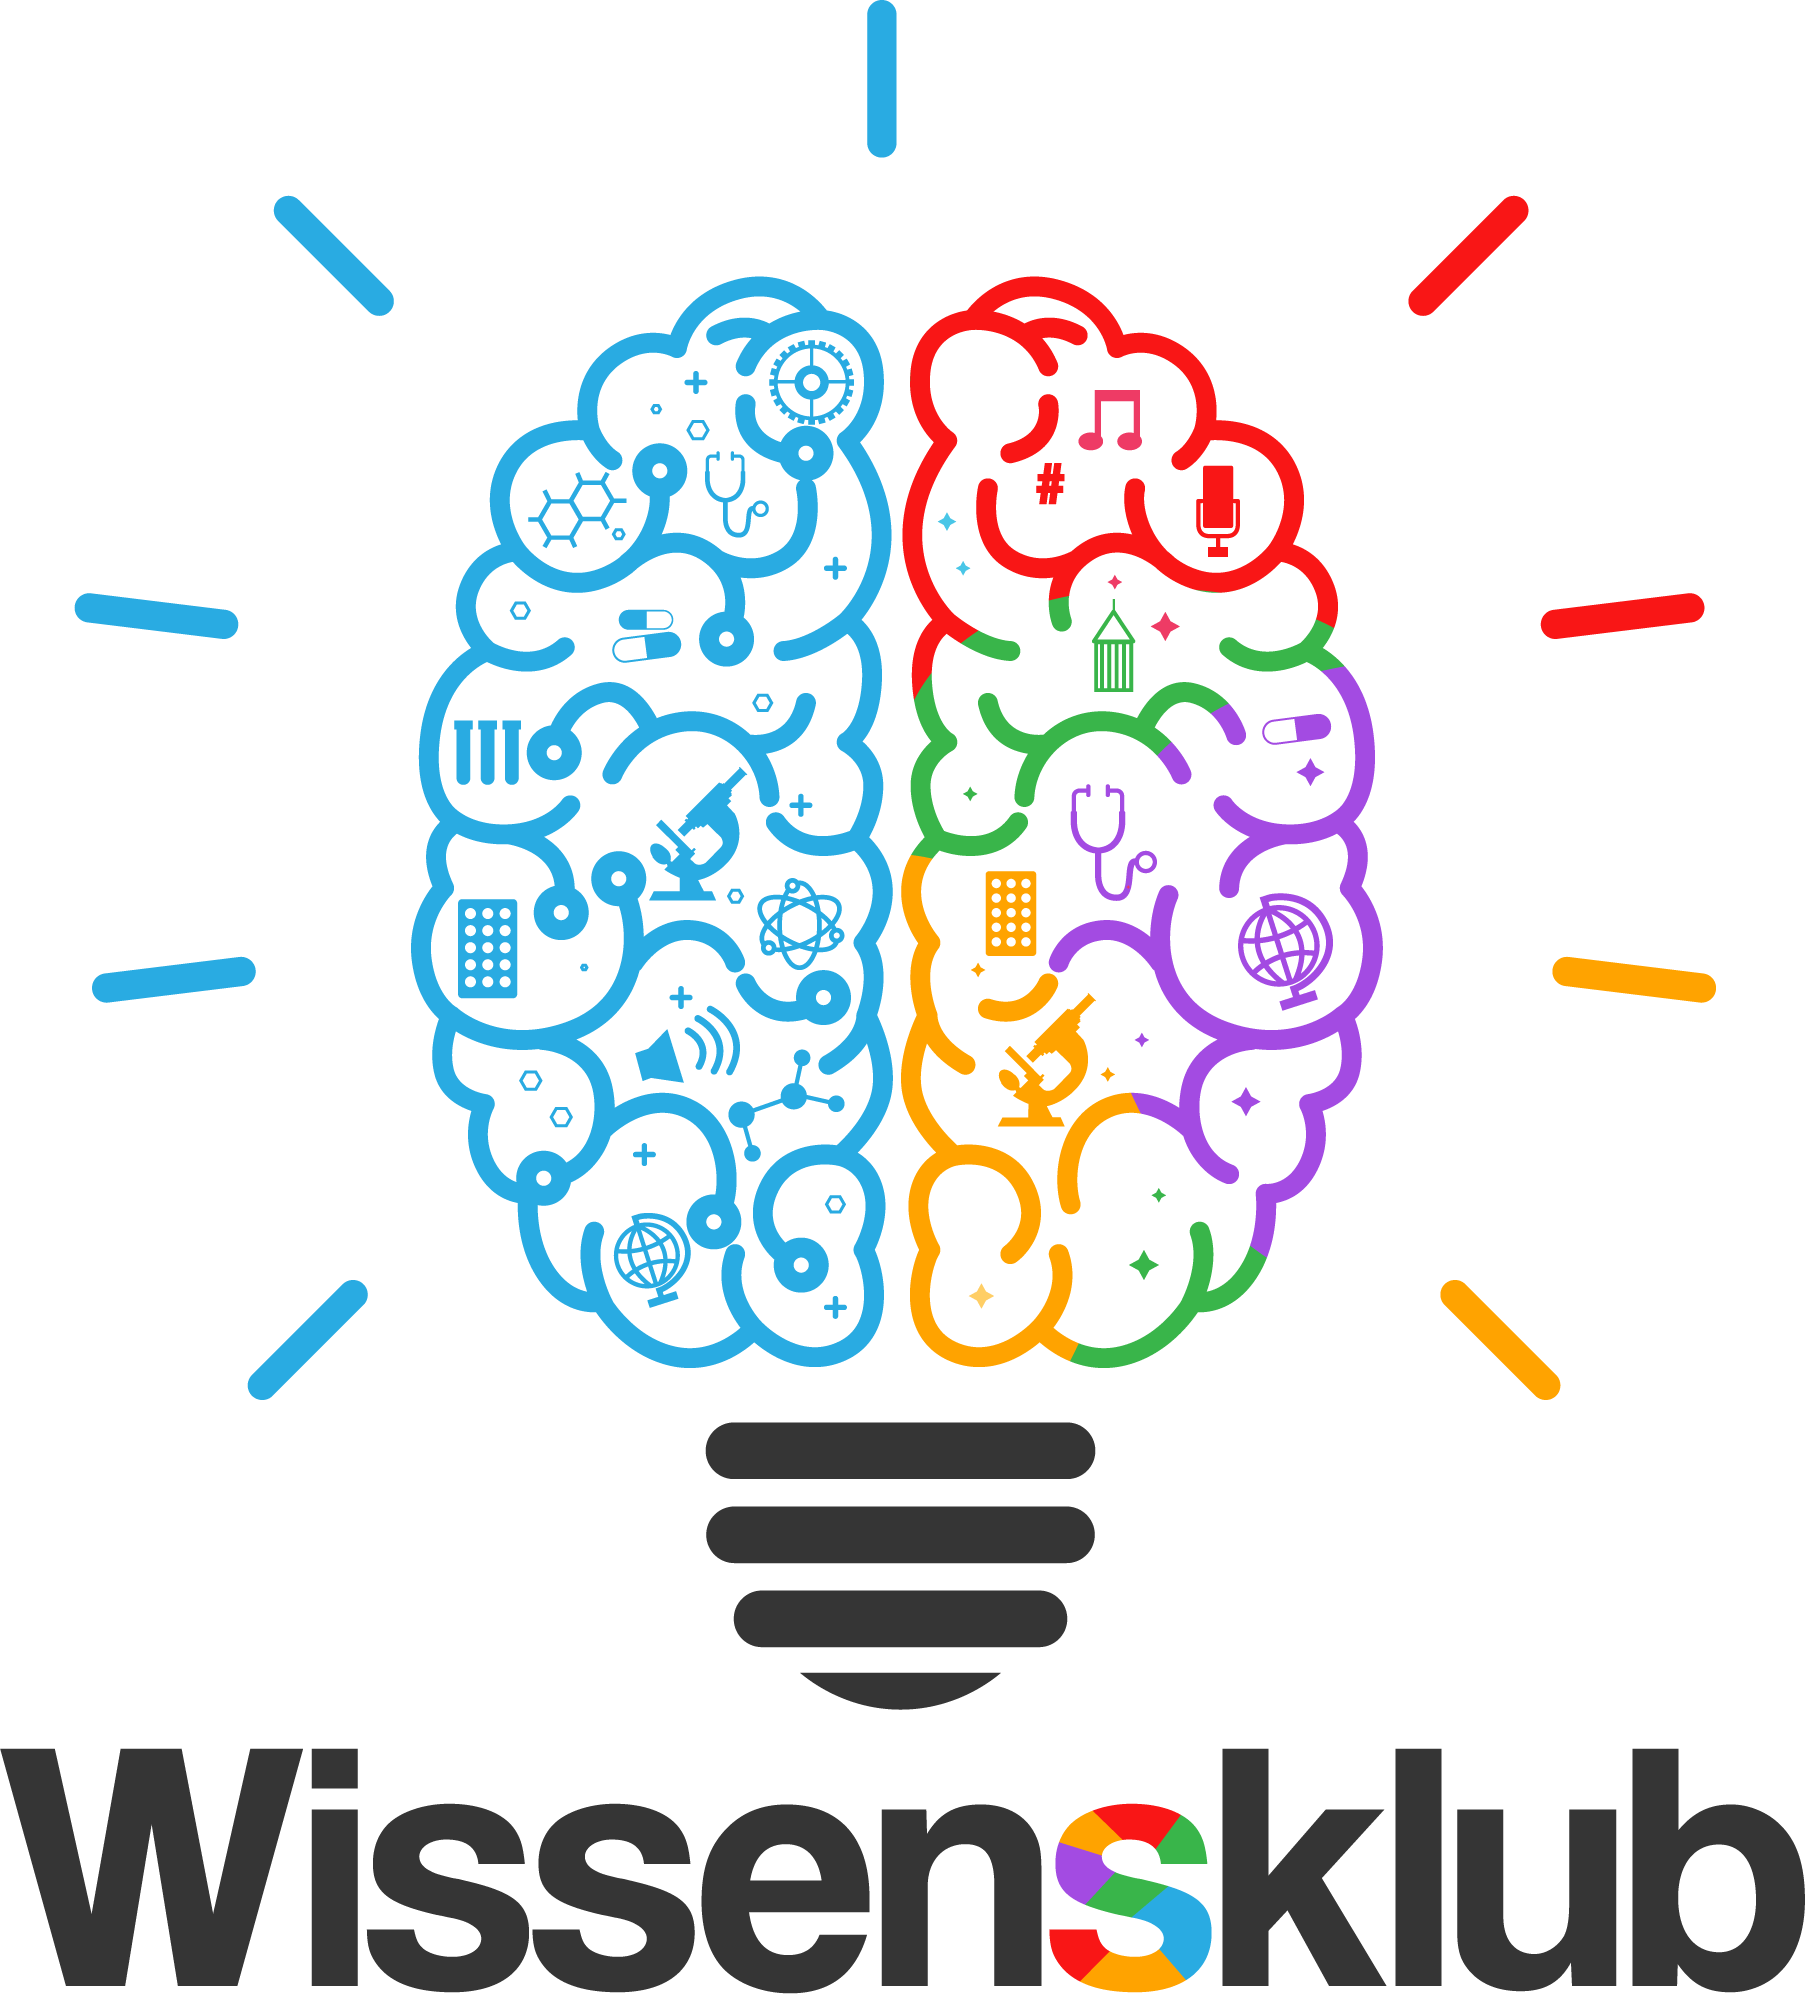
\includegraphics[height=3\baselineskip]{Wissensklub-Logo.png}
}
\addtolength{\headheight}{2\baselineskip}
\addtolength{\headheight}{0.61pt}
\fancyhead[C]{2024}

\begin{document}
\begin{titlepage}
    \begin{center}
        \vspace*{1cm}
            
        \Huge
        \textbf{Lernstandsübersicht}\\            
        \vspace{0.5cm}
        \LARGE
        Mathematik
            
        \vspace{1.5cm}
            
        \textbf{Wissensklub GmbH}
            
        \vfill
            
        Klasse 9\\
        \textit{Gymnasium} Nordrhein-Westfalen
            
        \vspace{0.8cm}
            
        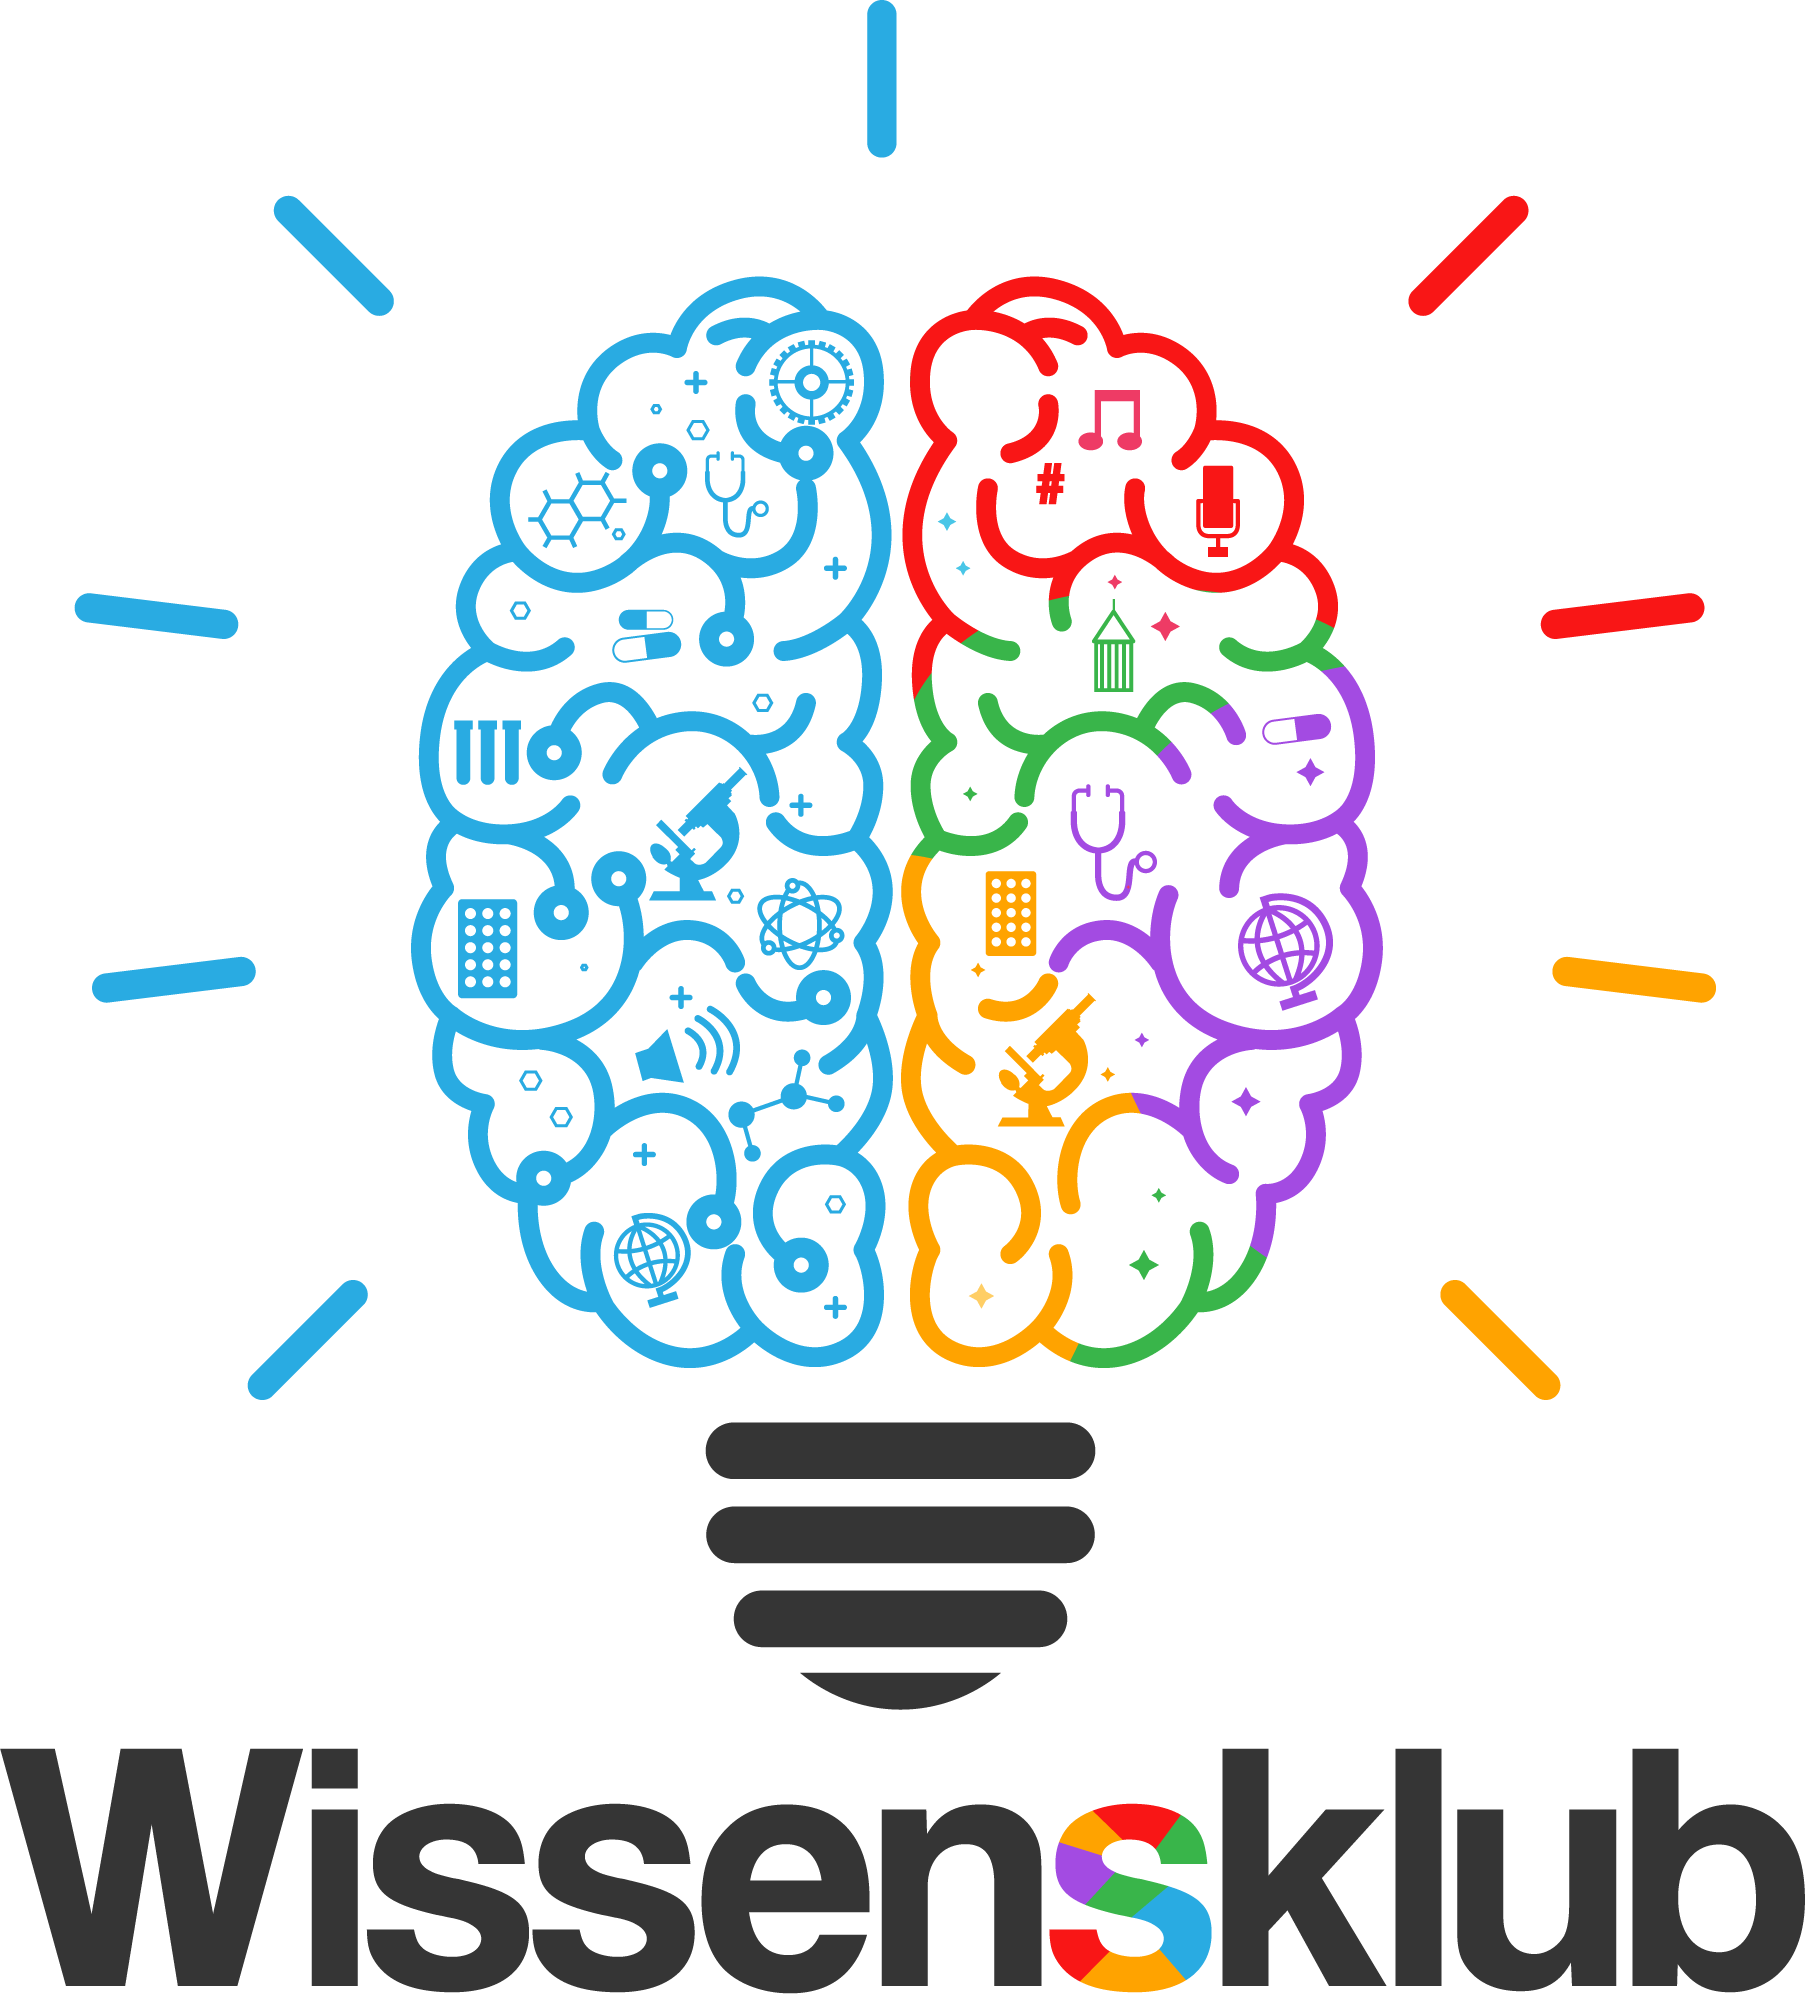
\includegraphics[width=0.5\textwidth]{Wissensklub-Logo.png}
            
        \Large
        2024          
    \end{center}
\end{titlepage}

\section{Reelle Zahlen}
Die bekannten Zahlen werden um die irrationalen Zahlen zu den reellen Zahlen erweitert.\\
\textbf{Voraussetzungen:}
\begin{itemize}
    \item \textbf{Rationale Zahlen}: natürliche, ganze und rationale Zahlen unterscheiden (Klassen 5-7)
    \item \textbf{Rechnen mit rationalen Zahlen:} Bruch-, Dezimal- und Prozentschreibweise (Klasse 7)
    \item \textbf{Quadrate}: Fläche von Quadraten berechnen (Klasse 5, 6)
    \item \textbf{Potenzen}: (Klasse 5, 6)
\end{itemize}
\subsection{Inhalte}
\subsubsection*{Quadratwurzeln}
Die Quadratwurzel $\sqrt{a}$ von $a$ ist diejenige positive Zahl, die quadriert $a$ ergibt: $(\sqrt{a})^2 = a$.
Es wird gelernt, das Quadrieren und Wurzelziehen (Radizieren) gegenteilig sind.
Quadratische Gleichungen, z.B. $x^2 = 9$ haben zwei Lösungen, eine positive und eine negative.
Es werden Wurzeln im Kopf berechnet, dabei werden natürliche aber auch rationale Zahlen benutzt.
Das Rechnen mit Wurzeln wird genutzt um quadratische Gleichungen zu Lösen.
Dieses Wissen wird auf das Rechnen mit Einheiten angewendet.
\subsubsection*{Wurzeln näherungsweise bestimmen}
Nicht jede positive Zahl hat eine Wurzel die wir leicht berechnen können. Durch geschicktes Rechnen können wir aber die Stellen dieser Wurzel annähern.
Wurzeln sollen auf dem Zahlenstrahl möglichst genau eingeordnet werden. Zwischen welchen natürlichen Zahlen liegt eine Wurzel?
Es werden Wurzeln auf eine gegebene Anzahl Nachkommastellen genau berechnet und  gerundet.
Dabei wird auch näherungsweise die Seitenlänge eines Quadrates berechnet.
Gegebenenfalls wird mit dem Heron-Verfahren ein Algorithmus zur näherungsweisen Bestimmung der Wurzel eingeführt.
\subsubsection*{Irrationale Zahlen}
Eine irrationale Zahl hat eine nichtabbrechende und nichtperiodische Dezimaldarstellung. Solche Zahlen lassen sich nicht als Bruch schreiben, sind also keine rationalen Zahlen.
Auf diese Zahlen stoßen wir, wenn wir z.B. $\sqrt{2}, \sqrt{3}$ berechnen.
Ein neuer Zahlenbereich, die reellen Zahlen werden eingeführt. Es soll zwischen diesen Zahlenbereichen unterschieden werden, und entschieden werden zu welchen Bereichen eine gegebene Zahl gehört.
Insbesondere soll zwischen rationalen und irrationalen Zahlen unterschieden werden.
\subsubsection*{Geschickt mit Wurzeln rechnen}
Es werden Rechengesetze zum Rechnen von Termen mit Wurzeln eingeführt. 
Wurzeln sollen mithilfe des Produkt- und Quotientengesetzes vereinfacht werden. Durch eine Zerlegung einer Zahl in ihre Faktoren können Wurzeln teilweise gezogen werden.
Das Distributivgesetz wird zusammen mit Wurzeln benutzt, um diese geschickt auszurechnen. 
\newpage
\section{Quadratische Funktionen}
Als wichtigen Typ von Funktionen werden quadratische Funktionen grafisch und algebraisch eingeführt.\\
\textbf{Voraussetzungen:}
\begin{itemize}
    \item \textbf{Funktionen}: grafisch zeichnen, Wertetabellen aufstellen und ablesen, Funktionsgleichungen aufstellen (Klasse 7-8)
    \item \textbf{Lineare Funktionen und Gleichungssysteme} (Klasse 8)
    \item \textbf{Binomische Formeln} (Klasse 8)
    \item \textbf{Funktionen im Sachkontext}: Modellierung und Lösen (Klasse 7-8)
\end{itemize}
\subsection{Inhalte}
\subsubsection*{$f(x) = a \cdot x^2$}
Diese Funktionen werden auch Parabeln genannt. Dem $n$-fachen des x-Wertes wird das $n^2$-fache als Funktionswert zugeordnet.
Die Form einer Parabel wird untersucht: Wann ist diese gestreckt/gestaucht, wann ist diese nach oben bzw. nach unten geöffnet?
Für Parabeln sollen Wertetabellen durch das Ausrechnen mehrerer Werte aufgestellt werden.
Mittels Wertetabelle sollen die Parabeln zeichnerisch in ein Koordinatensystem übertragen werden.
Für gegebene Punkte soll rechnerisch überprüft werden, ob diese auf dem Graph der Parabel liegen (Punktprobe). 
\subsubsection*{Scheitelpunktform quadratischer Funktionen}
Parabeln können wir im Koordinatensystem in $x$-Richtung verschieben. Diese Verschiebung lässt sich am leichtesten mit der Scheitelpunktform nachvollziehen.
Eine Parabel lässt sich ebenfalls in $y$-Richtung verschieben. Hier wird lediglich eine Konstante zu der Funktionsgleichung addiert.
Zu einer Funktion gegeben in Scheitelpunktform soll diese im Koordinatensystem gezeichnet werden (mit oder ohne Wertetabelle).
Für einen gegebenen Graphen einer Parabel soll der Scheitelpunkt abgelesen werden, und die Funktionsgleichung in Scheitelpunktform aufgeschrieben werden.
\subsubsection*{Normalform und quadratische Ergänzung}
Eine andere Darstellungsform einer quadratischen Funktionsgleichung ist die Normalform. Hier wird die Funktion als Summe der Variablen, geordnet nach Potenzen, festgehalten.
Durch das Vereinfachen des Terms ist es möglich die Scheitelpunktform in Normalform umzuwandeln.
Für das Umrechnen von Normalform in die Scheitelpunktform wird die quadratische Ergänzung eingeführt.
Zunächst soll zwischen den Darstellungsformen unterschieden und diese identifiziert werden. Vorteile dieser Formen werden besprochen
Bei einer Funktionsgleichung soll erkannt werden, welche Werte ergänzt werden müssen, um die binomische Formel anzuwenden (quadratische Ergänzung).
\subsubsection*{Aufstellen quadratischer Funtkionsgleichungen}
Quadratische Funktionen eignen sich zur Modellierung in vielen Zusammenhängen.
Je nach gegebenen Informationen eignet es sich die Scheitelpunktform oder die Normalform aufzustellen.
Es soll entschieden werden, je nach Informationen, welche Form genutzt wird und wie man damit die Funktionsgleichung bestimmt.
Quadratische Funktionen werden genutzt um geometrische Probleme zu lösen. Hier ist das Erweitern und Vereinfachen von Termen und binomische Formeln immer wieder im Einsatz
Aus Sachaufgaben sollen die wichtigen Informationen herausgefiltert werden, wie z.B. bestimmt Punkte oder der Schnittpunkt mit der y-Aschse oder der Scheitelpunkt.
\newpage
\section{Kreise, Prismen und Zylinder}
Es werden die bekannten drei-dimensionalen Figuren erweitert um Prismen.\\
\textbf{Voraussetzungen:}
\begin{itemize}
    \item \textbf{Rechnen mit Einheiten}: Längen, Flächen und Volumeneinheiten sind geläufig, Umrechnen in verschiedene Einheiten
    \item \textbf{Flächeninhalt \& Umfang}: Dreiecke, Quadrate, Rechtecke, Parallelogramme, Trapeze, \ldots  (Klasse 8)
    \item \textbf{Volumen \& Oberflächeninhalt}: Würfel, Quader 
    \item \textbf{Terme}: Terme vereinfachen und Gleichungen lösen (Klasse 7-8)
\end{itemize}
\subsection{Inhalte}
\subsubsection*{Kreisumfang und Kreisfläche}
Die Formeln für den Kreisumfang und die Kreisfläche, insbesondere die Kreiszahl $\pi$, werden hergeleitet.
Für gegebene Informationen, z.B. Durchmesser, Radius, Umfang, \ldots sollen die anderen Kennzahlen mit den bekannten Formeln hergeleitet werden.
Zusammengesetzte Flächen z.B. mit Kreisausschnitten sollen auf Umfang und Flächeninhalt untersucht werden.
Mit Aufgaben im Sachkontext sollen Probleme mit Kreisen analysiert werden.
\subsubsection*{Kreisteile}
Kreisteile lassen sich auf Umfang, Fläche und Bogenlänge untersuchen, wenn der Mittelpunktswinkel bekannt ist.
Daraus werden Formel für diese Kennzahlen von den Kreisformeln abgeleitet.
Wie im vorigen Thema sollen zusammengesetzte Flächen mit Kreisbögen untersucht werden.
\subsubsection*{Flächen bei Prismen und Zylindern}
Prismen sind Körper die durch die Verschiebung eines Vielecks im Raum entstehen. Prismen bestehen aus Grund- und Mantelfäche. Ist die Grundfläche ein Kreis, so wird das Prisma Zylinder genannt.
Durch das \textit{Aufklappen / Aufschneiden} des Prisma wird eine Formel für die Mantel- und Gesamtoberfläche hergeleitet.
Es soll bei einem gegebenem Prisma die Grund- und Mantelfäche identifiziert werden.
Je nach Art von Grundfläche soll der Flächeninhalt und Umfang berechnet werden können. Die Formel für Mantel- und Oberfläche soll anschließend angewendet werden können.
\subsubsection*{Volumen von Prismen und Zylindern}
Auch hier wird eine allgemeine Formel für das Volumen von Prismen hergeleitet. Dieses hat eine spezielle Form, falls das zugehörige Prisma ein Zylinder ist.
Diese Formel soll genutzt werden um das Volumen gegebener Prismen bzw. Zylinder auszurechnen.
Hier wird das Rechnen mit Längen- und Flächeneinheiten intensiv benutzt, welche vor Anwendung der Formeln entsprechend umgerechnet werden müssen.
An dieser Stelle wird ggf. das Prinzip von Cavalieri erarbeitet um das Volumen des Parallelepipeds (Dreidimensionales Parallelogramm) zu berechnen.

\newpage
\section{Potenzen und Potenzgesetze}
Potenzen sind hilfreich um große Zahlen lesbar darzustellen. Es werden mehrere Potenzgesetze erarbeitet um Terme mit Potenzen geschickt zu berechnen.
Insbesondere werden auch Potenzen mit nichtpositivem Exponenten vorgestellt.\\
\textbf{Voraussetzungen:}
\begin{itemize}
    \item \textbf{Potenzen}: Potenzen als wiederholte Multiplikation, natürliche Zahl im Exponent
    \item \textbf{Quadratwurzel}: Im Kopf berechnen, Rechengesetze geschickt anwenden(Klasse 8) 
    \item \textbf{Terme}: Terme mit mehreren Variablen vereinfachen und Gleichungen lösen, Rechengesetze (!) (Klasse 8)
\end{itemize}

\subsubsection*{Potenzen mit ganzzahligen Exponenten}
Eine Zahl $a^n$ mit natürlichem Exponenten $n$, steht für eine Multiplikation von $a$ $n$-mal mit sich selbst.
Bei $a^{-n}$ haben wir eine Multiplikation von $\frac{1}{a}$ $n$-mal mit sich selbst.
Es sollen die Werte solcher Potenzen berechnet werden und auch der Wert für Terme mit Variablen und solchen Potenzen.
Terme sollen schrittweise in der richtigen Reihenfolge aufgelöst und ausgerechnet werden.
\subsubsection*{Zahlen mit Zehnerpotenzen schreiben}
Aufgrund von der Struktur des Dezimalsystems lässt sich jeder Stelle eine Zehnerpotenz zuordnen.
Es wird die wissenschaftliche Schreibweise von Zahlen eingeführt. Zahlen in dieser Schreibweise sollen der Größe nach eingeordnet werden können.
Die Schüler sollen die Zahlen in die jeweils andere Schreibweise überführen.
\subsubsection*{Potenzen mit gleicher Basis}
Wenn Potenzen mit gleicher Basis multipliziert oder dividiert werden, ändert sich lediglich der Exponent. Diese Erkenntnis wird als Potenzgesetz festgehalten.
Damit sollen Potenzen verrechnet werden und das Ergebnis ggf. als Dezimalzahl oder Bruch ausgerechnet werden.
Fehler in Termumformungen mit Potenzen sollen nachvollzieht werden können.
Terme bestehend aus Summen und Produkten von Potenzen sollen vereinfacht und ausgerechnet werden.
\subsubsection*{Potenzen mit gleichem Exponenten}
Die Basis kann bei Produkten und Quotienten von Potenzen zusammengefasst werden; dies stellt das zweite Potenzgesetz dar.
Hier sollen ebenfalls Terme in diesem Zusammenhang vereinfacht und ausgerechnet werden.
Terme die Potenzen mit gleicher Basis und/oder Exponenten benutzen werden intensiv genutzt.
\subsubsection*{Potenzieren von Potenzen}
Werden Potenzen potenziert, so multiplizieren sich die Exponenten und fallen zu einer einzelnen Potenz zusammen.
Mit diesen drei Potenzgesetzen lassen sich verschachtelte Terme bauen und sollen vereinfacht und berechnet werden.
\subsubsection*{Potenzen mit rationalen Exponenten}
Aus dem Kontext der Quadratwurzeln werden Potenzen mit rationalem Exponenten, hier $\frac{1}{2}$, eine sinnvolle Interpretation gegeben.
Hier sollen Wurzeln in Potenzen und andersrum umgewandelt werden.
Damit lassen sich mittels der Potenzgesetze auch n-te Wurzeln berechnen.
\newpage
\section{Satz des Pythagoras und Körper}
Mit dem Satz des Pythagoras lassen sich die Seiten eines rechtwinkligen Dreiecks besser verstehen. Insbesondere zum Berechnen fehlender Seitenlängen einer Fläche oder im Raum wird dieser praktisch.\\
\textbf{Voraussetzungen}:
\begin{itemize}
    \item \textbf{Flächen \& Umfänge}: Rechtecke, Dreiecke, Trapeze, Kreise
    \item \textbf{Wurzel}: berechnen und vereinfachen (Klasse 8) 
    \item \textbf{Oberfläche \& Volumen}: Prismen, Zylinder
    \item \textbf{Terme mit Variablen}: Formeln mit unbekannten Größen berechnen, nach verschiedenen Variablen umstellen(Klasse 8)
\end{itemize}

\subsection{Inhalte}
\subsubsection*{Der Satz des Pythagoras}
Der Satz des Pythagoras stellt den Zusammenhang der Längen der Katheten und der Hypothenuse her.
Es soll am Dreieck erkannt werden, ob dieses rechtwinklig ist und wo die Katheten und die Hypothenuse liegt.
Mit dem Satz des Pythagoras soll ein Dreieck rechnerisch auf Rechtwinkligkeit überprüft werden. 
Je nachdem welche Werte gegeben sind, soll die Formel umgestellt werden um die fehlenden Größen zu ermitteln.
\subsubsection*{Pythagoras in Figuren und Körpern}
In einer dreidimensionalen Figur, z.B. einem Quader, lassen sich mit der Raumdiagonale rechtwinklige Dreiecke finden.
Für Quader, Pyramiden, Prismen soll der Satz des Pythagoras genutzt werden, um fehlende Größen zur Berechnung des Rauminhalts oder der Oberfläche zu finden.
Hier ist ein guter Umgang mit Schrägbildern und eine sehr gute geometrische Vorstellungskraft erforderlich.

\subsubsection*{Pyramiden}
Pyramiden können entweder eine dreieckige oder rechteckige Grundfläche haben. Es wird für das Volumen und den Oberflächeninhalt eine Formel hergeleitet.
Diese Formeln sollen genutzt werde um Kennwerte zu berechnen, oder fehlende Seitenlängen oder die Höhe nach Umstellen der Formel zu ermitteln.

\subsubsection*{Kegel}
Die Herleitung der Pyramidenformeln kann angepasst werden um diese auf den Kegel zu übertragen.
Auch hier stellen sich die gleichen Schwierigkeiten und Aufgabentypen wie bei der Pyramide.
\subsubsection*{Kugeln}
Wie in den vorigen Kapiteln wird eine Formel für das Volumen und dne Oberflächeninhalt einer Kugel hergeleitet.
Die Formel soll genutzt werden um fehlende Kenngrößen zu ermitteln, gegebenenfalls muss diese zuvor umgestellt werden.
Mit den verschiedenen neuen Körpern können zusammengesetzte Figuren erzeugt werden, dessen Oberfläche und Volumen berechnet werden soll.
Die erarbeitetetn Körper können in den Sachkontext eingesetzt werden um reale Formen zu modellieren und Probleme zu kösen.

\end{document}